\documentclass[10pt,slovak,a4paper]{article}

\usepackage[slovak]{babel}
\usepackage[IL2]{fontenc} 
\usepackage[utf8]{inputenc}
\usepackage{graphicx}
\usepackage{url}
\usepackage{hyperref}
\usepackage{xurl}
\usepackage{cite}
\usepackage{float}
\usepackage{amsmath}

\title{Algoritmy odporúčania filmov v Netflix\thanks{Semestrálny projekt v predmete Metódy inžinierskej práce, ak. rok 2024/25, vedenie: Ing. Richard Marko, PhD}}

\author{Yehor Bohuslavskyi\\[2pt]
	{\small Slovenská technická univerzita v Bratislave}\\
	{\small Fakulta informatiky a informačných technológií}\\
	{\small \texttt{xbohuslavkyi@stuba.sk}}
	}

\date{\small 9. december 2024}

\begin{document}

\begin{figure}[h!]
  \centering
  
\includegraphics[width=\textwidth]{Images_tables/fiit_logo.png} 
\end{figure}

\maketitle

\begin{abstract}
Túto tému som si vybral, pretože je veľmi zaujímavé, ako technológie a umelá inteligencia(ktorá je v súčasnosti jednou z najrozvíjajúcejších sa tém) ovplyvňujú naše každodenné rozhodovanie o tom, čo sledujeme. Ja som zvedavý, že ako po zhliadnutí jedného tureckého filmu, ktorý som ani neohodnotil, sa mi v odporúčaniach začali objavovať podobné filmy. 

V systéme sa nachádza viac, ako 15 000 filmov a zobrazuje vám len tie, ktoré sa vám budú páčiť (neskôr dozvieme sa, ako to funguje). Fakt: ani jeden používateľ Netflix nebol by schopný si samostatne nájsť film alebo seriál, ktorý by sa mu páčil bez požívania algoritmu odporúčania filmov.\cite{Netflix:Algorithm}
 
V tomto článku sa podrobne pozrieme na algoritmy spoločnosti Netflix. V súčasnosti je systém Netflix postavený na algoritme, ktorý využíva umelú inteligenciu a strojové učenie. Pozrieme sa aj na umiestnenie odporúčaní na obrazovke, kde je niekoľko typov návrhov. Prvým je „Odporúčané pre vás“, po ňom idú „Trendy“, na stránke sa nachádza aj záložka „New Releases“.\cite{Netflix:Recommendation:System}
Podrobne sa pozrieme aj na filtračné algoritmy, ktoré sa delia na dva hlavné typy.\cite{Fil:alg:typy} Akú rolu odohrávajú hodnotenia a správania používateľov v rámci algoritmu „collaborative filtering“ a „filtrovanie na základe obsahu“.

Zaujímavým aspektom sú aj systémy hodnotenia. Patrí medzi ne „Personalizované hodnotenie videa (PVR)“, „Top-N Ranking“, „Rebríček obľúbených filmov“ a „Zoznam zaujímavého obsahu na neskoršie sledovanie“. Každé z týchto hodnotení je personalizované pre jednotlivých používateľov, čo je veľmi zaujímavé.

V rámci článku sa budeme venovať aj typom údajov, ktoré Netflix používa. Tie sa zhruba delia na dva typy: základné typy zhromažďovaných údajov a dodatočné informácie. Medzi základné patria „interakcie používateľa so stránkou“, ktoré pozostávajú z histórie sledovania a hodnotení. Druhým typom sú „korelačné údaje“, „informácie o obsahu knižnice Netflix“, ako napríklad žánre. Ďalšie uvidíme ako ovplyvňujú  špecifickejšie typy informácií, ako sú napríklad denný čas, používané zariadenie alebo priemerná dĺžka sledovania.

\end{abstract}

\section{Úvod}
Cieľom spoločnosti Netflix je používať odporúčacie algoritmy na maximalizáciu spokojnosti
používateľov. Hlavným cieľom je prispôsobiť obsah každému jednotlivému používateľovi.

Netflix má obrovskú knižnicu obsahu a obmedzené rozhranie obrazovky, čo veľmi sťažuje odporúčanie relevantného obsahu, a každý používateľ má iný vkus, preferencie a zvyky pri sledovaní, takže personalizácia musí byť veľmi presná.
Čo robí Netflix na dosiahnutie tohto cieľa, sa dozviete po tomto článku.

\section{Technológie a Umelá inteligencia v Netflix}
Na zlepšenie používateľského zážitku, Netflix využíva umelú inteligenciu a strojové učenie. Medzi kľúčové aplikácie týchto technológií patrí\cite{AI}

\begin{enumerate}
    \item \textbf{Odporúčania obsahu}: na základe vašich zvykov a preferencií algoritmy spoločnosti Netflix môžu vám ponúknuť personalizované odporúčania. Analýza údajov obsahuje aj žáner a obľúbenosť obsahu.\cite{Odp:alg:sys}
    
    \item \textbf{Personalizované miniatúry}: Ak si zoberieme ako príklad film „Shadow and Bone“, miniatúry filmu sú prispôsobené vašim záujmom a môžu používať obrázky zobraté s iných populárnych programov, skrátka čokoľvek, čo upúta vašu pozornosť.\cite{AI_deep:lerning}
    
    \item \textbf{Kvalita streamovania}: Na zabezpečenie plynulého prehrávania videa využíva Netflix údaje na predpovedanie preťaženia siete a ukladá obsah do medzipamäte na blízkych serveroch, takže si môžete vychutnať filmy bez oneskorenia.\cite{AI_deep:lerning}
    
    \item \textbf{Kontrola kvality obsahu}: Pred odporúčaním nového obsahu používateľom prechádza niekoľkými fázami testovania vrátane zvuku a obrazu, aby boli všetci používatelia spokojní.\cite{AI_deep:lerning}
    
\end{enumerate}

Táto technológia nielenže zvyšuje spokojnosť používateľov, ale podporuje aj dlhodobú angažovanosť.

\begin{figure}[H]
  \centering
  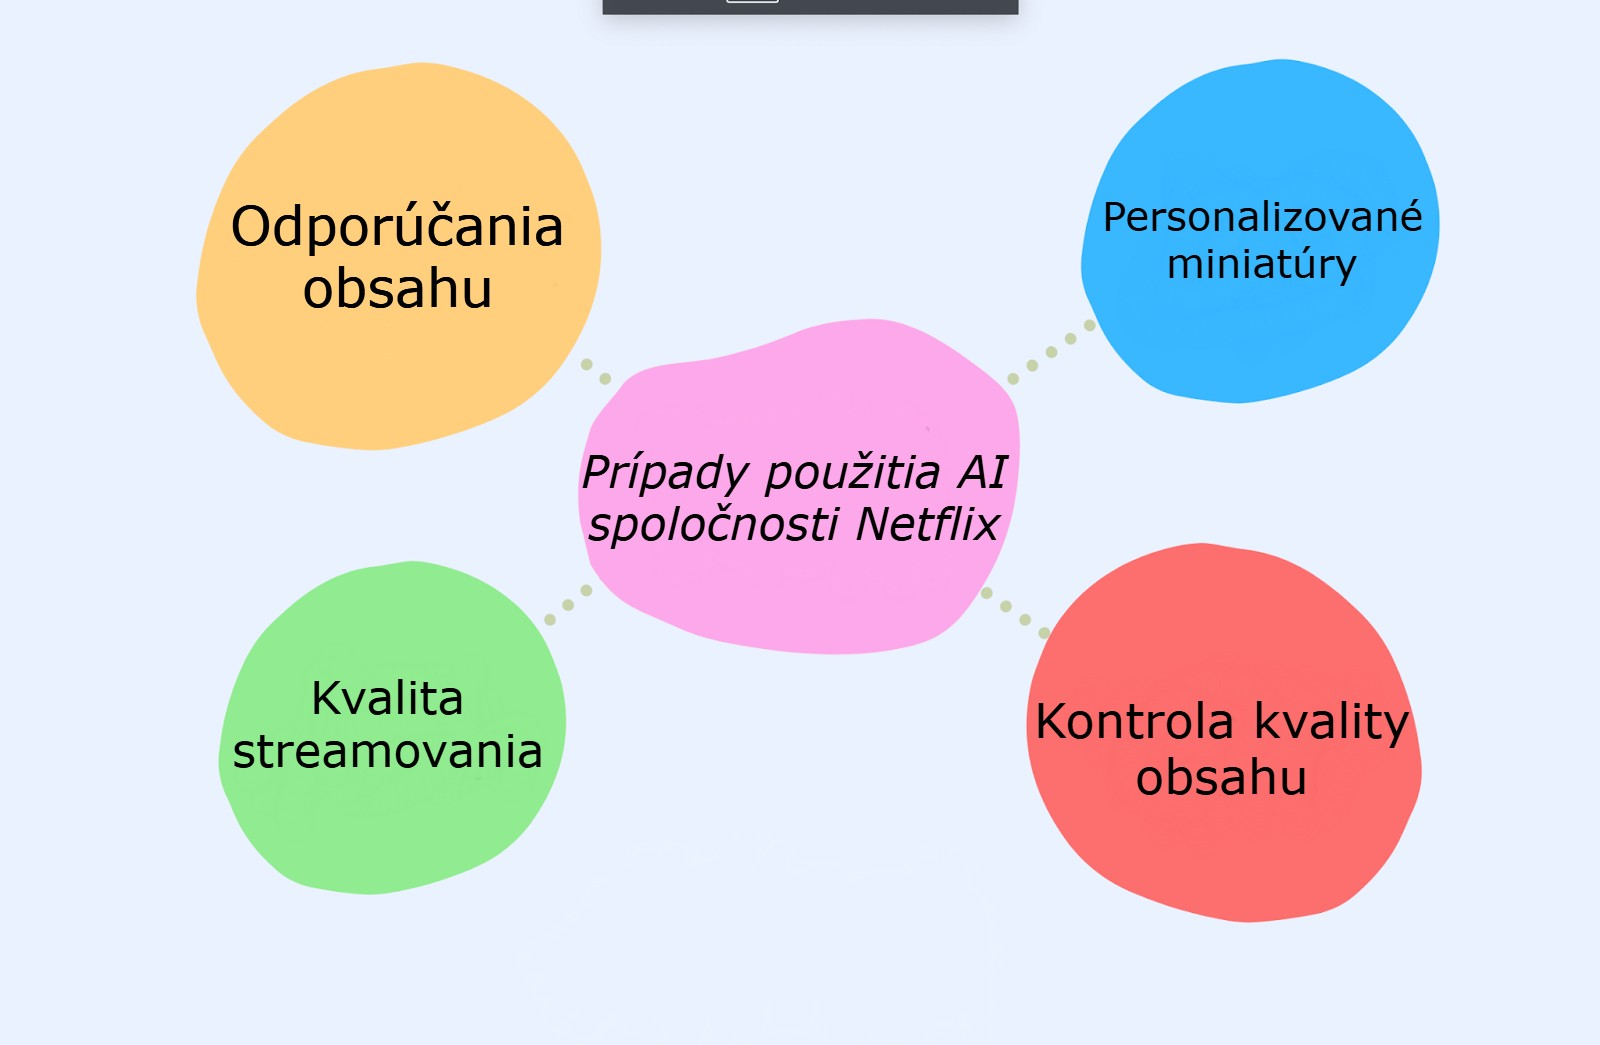
\includegraphics[width=1\textwidth]{Images_tables/AI.jpg}
  \caption{Systém umelej inteligencie}
\end{figure}


\section{Typy Odporúčaní na Netflix}

\begin{enumerate}
    \item \textbf{Odporúčania obsahu}: na základe vašich zvykov a preferencií vám algoritmy spoločnosti Netflix môžu ponúknuť personalizované odporúčania. Analýza údajov zahŕňa aj žáner a obľúbenosť obsahu.\cite{Odp:sys}
    
    \item \textbf{Kolaboratívne filtrovanie}: vytvorením skupín používateľov, ktorí majú podobný vkus, a na základe správania a preferencií používateľov táto metóda navrhuje obsah, ale má problém so studeným štartom.\cite{Chladny:start}
    
    \item \textbf{Filtrovanie na základe obsahu}: tento typ filtrovania zhromažďuje údaje, napríklad aký žáner filmu preferujete, akého režiséra alebo akých hercov uprednostňujete, a odporúča vám podobný obsah.
    
    \item \textbf{Hybridné modely}: tento typ kombinuje kolaboratívne filtrovanie a filtrovanie založené na obsahu, pretože len tak sa dá vyriešiť problém studeného štartu.

    \item \textbf{Odporúčania založené na hlbokom učení}: používajú sofistikované algoritmy umelej inteligencie, ktoré modelujú interakciu používateľa ako postupný rozhodovací proces.
\end{enumerate}    

\begin{figure}[H]
  \centering
  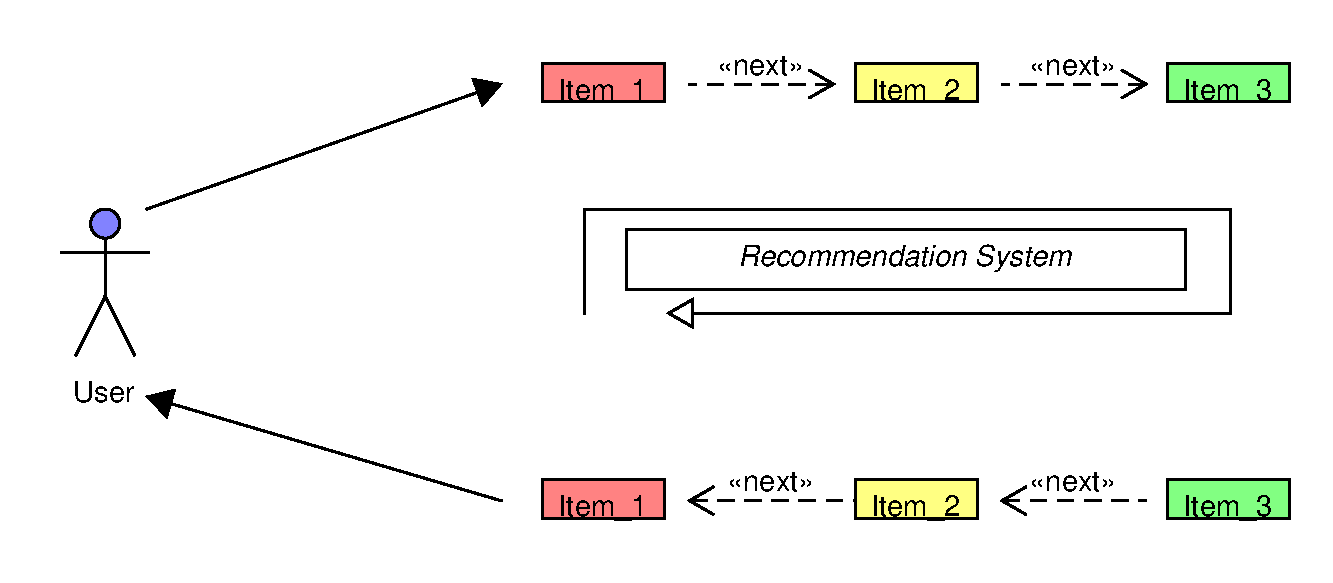
\includegraphics[width=1\textwidth]{Images_tables/RecommendationSystem_pdf.pdf}
  \caption{Systém odporúčaní}
\end{figure}

\section{Filtračné algoritmy}

Netflix používa rôzne typy filtrovania, ako je kolaboratívne filtrovanie, filtrovanie na zaklade obsahu\cite{Filtracne:algoritmy}, hybridné modely alebo odporúčania založené na hlbokom učení, ale v tomto článku sa budeme zaoberať len prvými dvoma, pretože sú najpoužívanejšie. 
Rozdiel medzi nimi spoznáte podľa názvu, ale poďme sa na ne pozrieť bližšie.

\textbf{Kolaboratívne filtrovanie} je algoritmus, ktorý sleduje, aké sú vaše preferencie pri výbere filmov, a na základe týchto údajov vás zoskupí s ostatnými ľuďmi, ktorí majú podobný vkus. Algoritmus využíva matematické modely na hodnotenie podobnosti a predikciu preferencií. Jedným z príkladov výpočtu skóre podobnosti môže byť vzorec: 
\[
\frac{\arcsin^2(x)}{2} - \frac{\sqrt{1 - x^2} \cdot (x^2 + 2)}{3} + C
\]
Tu \textbf{x} predstavuje normalizovanú hodnotu pre konkrétny atribút alebo interakciu používateľa, zatiaľ čo \textbf{C} je konštanta upravujúca celkové skóre. Takéto výpočty pomáhajú algoritmu rozhodnúť, ktoré filmy alebo seriály budú odporučené používateľovi. Názornejšie, ako funguje, nájdete na \hyperref[U:I]{Obr.3}, kde je graficky znázornená metóda kolaboratívneho filtrovania. Hoci sú na obrázku len 2 ľudia, v skutočnosti ich môže byť 100 alebo viac.\cite{Coll:fil} Hlavným problémom tohto systému je problém studeného štartu, ktorý sa objavuje ako dôsledok nedostatku údajov o používateľovi alebo filmoch v systéme. Tento problém sa rieši použitím niekoľkých typov filtrovania, ale Netflix sa naďalej snaží tento problém vyriešiť. Metóda kolaboratívneho filtrovania sa delí na dve ďalšie metódy, prvou je kolaboratívne\textbf{filtrovanie založené na používateľovi}(v tabulke oznacene ako UBCF), zameriava sa na vyhľadávanie ľudí s podobným vkusom ako vy.\cite{Fil:alg:colab} Ako presne? Najprv vypočíta podobnosť medzi všetkými používateľmi a v závislosti od výsledku začne odporúčať filmy, ktoré ste ešte nevideli, pričom sa páčia ľuďom s podobným vkusom.
Druhou čiastkovou metódou je kolaboratívne\textbf{filtrovanie založené na položkách}(IBCF), líši sa tým, že nehľadá podobnosti medzi ľuďmi, ale medzi položkami, s ktorými ste komunikovali, a odporúča podobné. Ak sa vám napríklad páči film, v ktorom hral Robert Downey Jr, systém vám začne odporúčať filmy alebo seriály, v ktorých hral tento herec.
Podrobnejšie, aký je medzi nimi rozdiel a aké aspekty zahŕňajú, si môžete pozrieť v nasledujúcej tabuľke.

\begin{figure}[H]
  \centering
  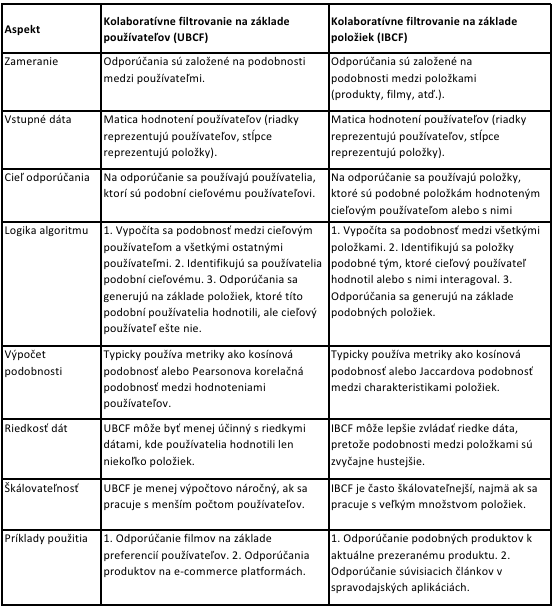
\includegraphics[width=1\textwidth]{Images_tables/table_filtering.png} 
  \label{U:I}
  \caption{UBCF/IBCF}
\end{figure}

\textbf{Filtrovanie na zaklade obsahu} tento typ filtrovania je veľmi ľahko pochopiteľný, pretože podstatou algoritmu je odporučiť obsah, ktorý je podobný predchádzajúcim výberom používateľa, \hyperref[Types:of:filtering]{Obr.4}. Algoritmus venuje pozornosť charakteristikám, ako sú „názov“, „krajina“, „režisér“, „obsadenie“, „uvedené“ a „opis“ filmu/seriálu, aby odporučil filmy, ktoré zodpovedajú vášmu vkusu.\cite{Fil:obsah} Ak napríklad radi sledujete komédie, Netflix vám začne odporúčať filmy s Jackie Chanom alebo komédie s inými populárnymi hercami. Algoritmus tiež uvidí, že máte radi filmy s Jackie Chanom, a začne odporúčať filmy súvisiace s východnou kultúrou, a tak Netflix postupne zachytí vaše preferencie a bude sa stále zlepšovať. Najväčším problémom tohto typu filtrovania je monotónnosť obsahu. V dôsledku toho používateľ stráca záujem o sledovanie filmov na tejto platforme.\cite{Fil:alg:obsah}

\begin{figure}[h!]
  \centering
  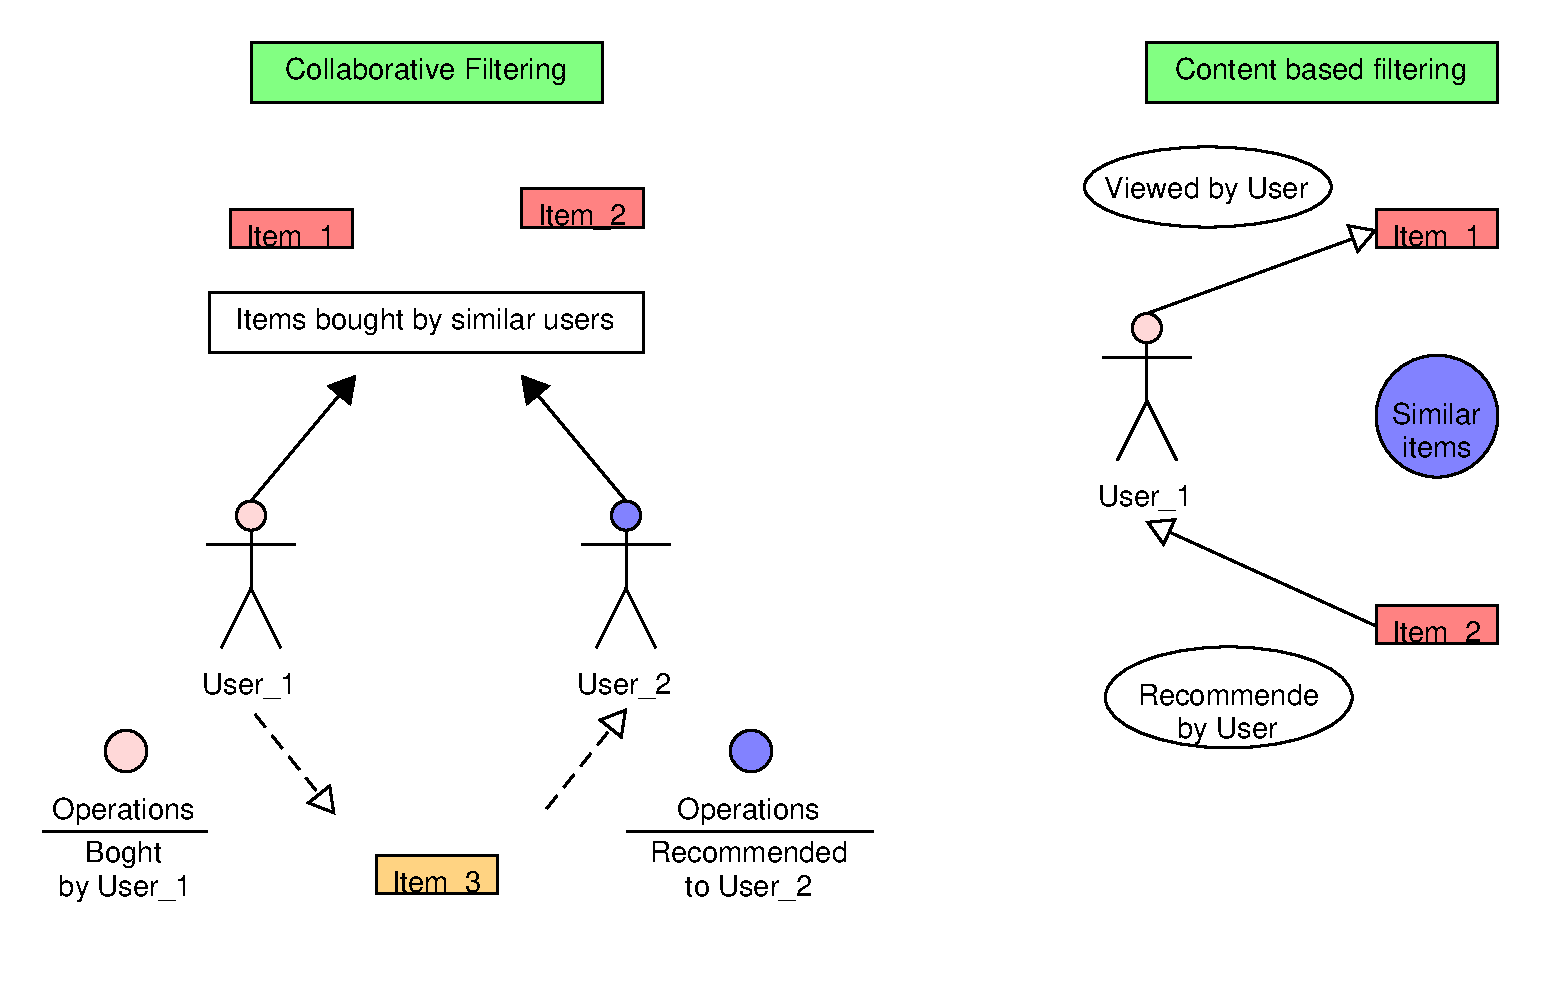
\includegraphics[width=1\textwidth]{Images_tables/Filtering_pdf.pdf}
  \label{Types:of:filtering}
  \caption{Typy filtrovania}

\end{figure}

\section{Systémy Hodnotenia}
 Kľúčovými zložkami odporúčacieho systému spoločnosti Netflix je niekoľko personalizovaných systémov hodnotenia, z ktorých každý je navrhnutý tak, aby zohľadňoval rôzne aspekty zvykov používateľa pri sledovaní. Poďme sa do týchto systémov ponoriť a preskúmať, ako fungujú.
\begin{enumerate}
    \item \textbf{Personalizovaný rebríček videí (PVR)} je jedným z najmodernejších  nástrojov hodnotenia, ktoré Netflix používa.\cite{Hodnotenie} Pretože nielen chápe správanie používateľov v minulosti, ale dokáže predpovedať aj budúce potreby. Aby sme lepšie porozumeli tomuto algoritmu, pozrime sa, ako funguje. V prvom rade je založený na systéme hlbokého učenia a neustále sa prispôsobuje používateľovi. Základnou myšlienkou je použiť historické údaje (napríklad zvyky používateľov) na určenie vašich zvykov a uprednostnenie obsahu, ktorý vás zaujíma. Celkovo systém používa personalizované údaje používateľa na poskytnutie celkového relatívneho poradia položiek v rade.

    \item \textbf{Systém Top-N Ranking} je založený na kombinácii kolaboratívneho a obsahového filtrovania. Ako už názov napovedá, poskytuje najlepšie hodnotené filmy, ktoré zodpovedajú vkusu používateľa. Je podobný ako PVR s tým rozdielom, že sa pozerá len na hodnotenie titulu. Netflix využíva Tento algoritmus aj na doplnenie riadkov, ako napríklad  “Pre teba“.

    \item\textbf{Obľúbene medzi používateľmi}, ktorý predpovedá časové trendy na základe globálnych a regionálnych údajov o filmoch a televíznych seriáloch. Vo všeobecnosti existujú dva typy trendov: sezónne a špeciálne.Na základe názvu by ste mohli predpokladať, že čo je čo, ale poďme sa na ne pozrieť bližšie.
    
    Do sekcie \textbf{sezónnych trendov} sa zvyčajne zaraďujú filmy ako “Sám doma“ alebo “Polárny expres“, pretože získavajú popularitu v období Vianoc, alebo horory počas Halloween.

    Sekcia \textbf{špeciálne} alebo \textbf{krátkodobé} udalosti môže patriť Pandémiu 2021, ktorá zaznamenala nárast populárnosti dokumentárnych filmov a filmov o infekciách.

    \item \textbf{Pozrite sa neskôr}, ide o pomerne zaujímavý algoritmus, ktorý je založený na dvoch kľúčových bodoch. Prvým je, že do tejto časti patria filmy, ktoré ste ešte nedopozerali, zvyčajne televízne seriály s niekoľkými sezónami, ale môžu to byť aj filmy alebo seriály, ktoré ešte neboli dokončené. A druhým bodom je, že na základe regionálnych údajov a pomocou kolaboratívneho filtrovania algoritmus zmieša vaše nepozerané filmy s podobnými filmami, ktoré sa páčia iným používateľom.
    
\end{enumerate}

Po tom, ako algoritmy analyzujú vás a vaše správanie, začnú vytvárať vaše personalizované odporúčania, krok za krokom prostredníctvom všetkých parametrov, čo je graficky znázornené na  \hyperref[Ranking]{Obr.5} plynulo prechádzajú z backendu na frontend, takýto proces sa nazýva \textbf{generovanie stránok}.

\begin{figure}[h!]
  \centering
  \label{Ranking}
  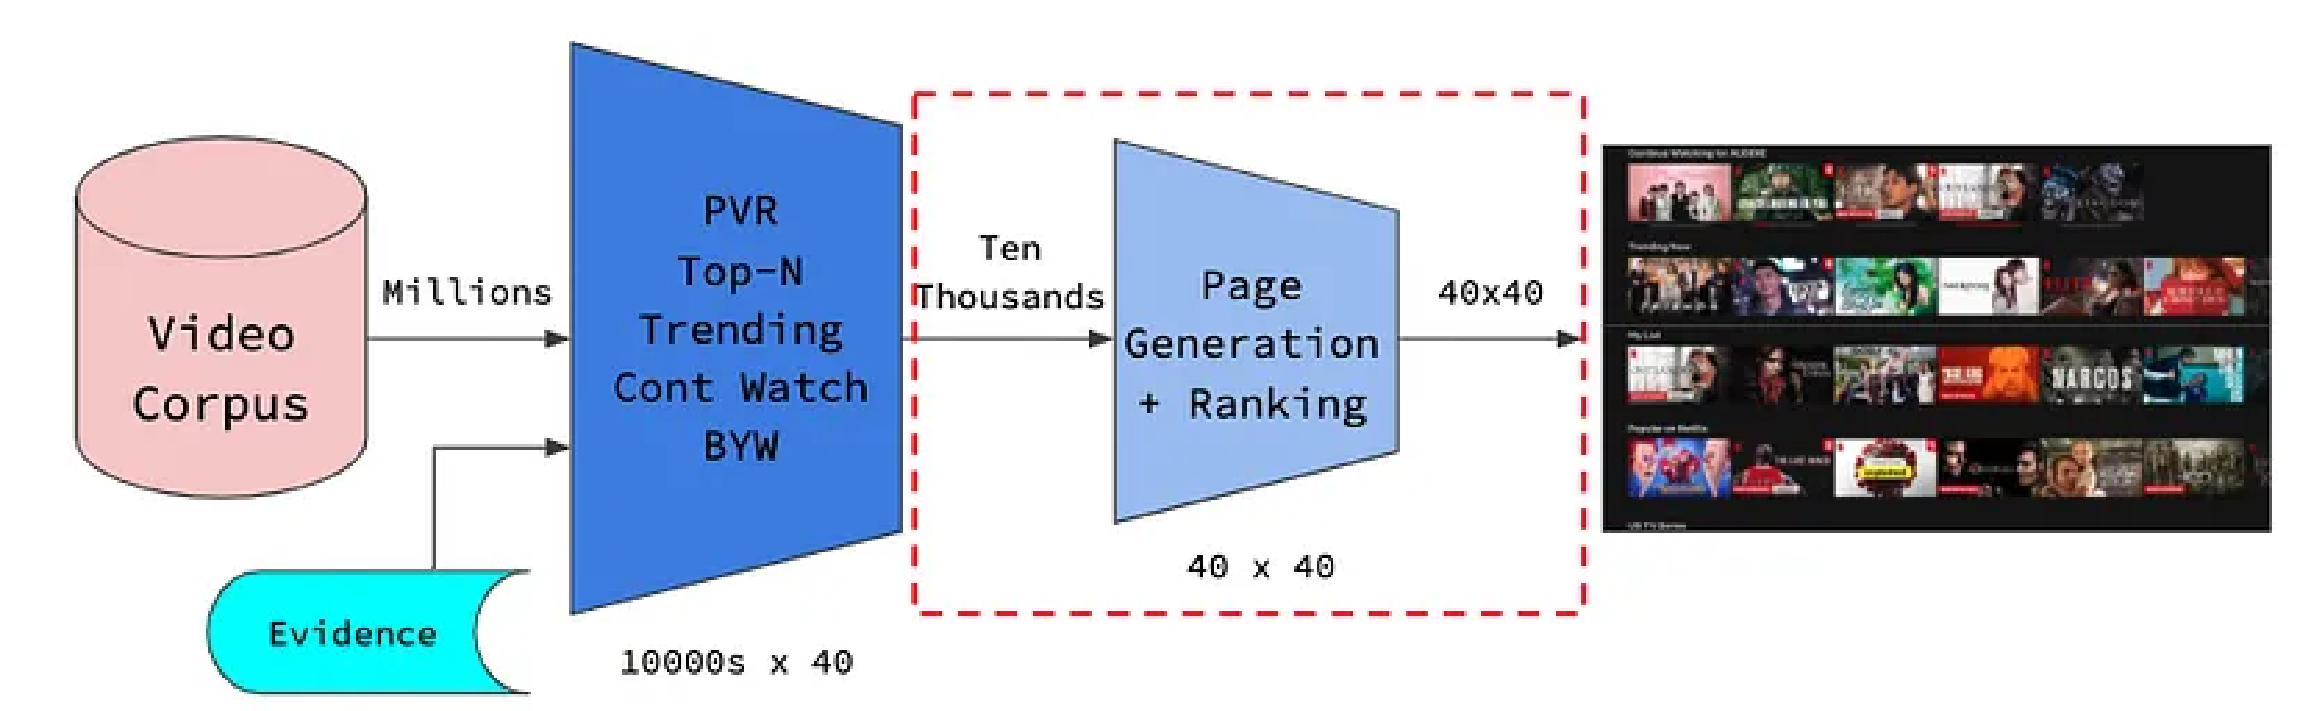
\includegraphics[width=1\textwidth]{Images_tables/Ranking.pdf}
  \caption{Hodnotenie}
\end{figure}

\section{Typy Údajov v Netflix}
A teraz nehovoríme len o tom, aké filmy uprednostňujete, ale o výsledkoch systému, ktorý má viac ako 1 300 skupín odporúčaní skenujúcich vás a vaše zvyky. Netflix vie, že máte radi nielen thrillery, on vie ze zaoberáte sa psychologické thrillery so silnými ženskými hrdinkami, ktoré sledujete väčšinou cez víkend večer. Asi vás zaujíma ako, odpoveď nájdete v tejto časti.

\begin{enumerate}
    \item \textbf{Údaje o účtoch a predplatnom}, na prvý pohľad nie je jasné, prečo Netflix používa tieto údaje, ale je to na lepšiu správu vašich účtov a zaistenie bezpečnosti monitorovaním vašej aktivity na účte.

    \item \textbf{Zariadenie} a \textbf{dáta}, z ktorého sledujete filmy a v akom čase, aby sú vedeli, čo a kedy vám máme odporučiť.\cite{Data} Vezmime si, že v práci počas prestávky dve hodiny pozeráte komediálne seriály a potom skončí a večer si na televízore zapnete Netflix, kde pozeráte horory, zhromažďovaním týchto informácií sa vaše odporúčania začnú meniť podľa dátumu a času.

    \item Spoločnosť Netflix zhromažďuje údaje ob  \textbf{históriu dopytov}, aby mohla sledovať trendy a prispôsobovať ponuky obsahu s cieľom zdôrazniť to, čo používatelia hľadajú.

    \item Samozrejme, že spracúvajú \textbf{hodnotenie obsahu} a \textbf{spätnú väzbu} používateľov, aby pochopili kvalitu a hodnotenie obsahu a rozhodli sa, či obsah spracovať alebo odstrániť.
    
\end{enumerate}

\section{Záver}
Toto je koniec článku a stojí za to ho zhrnúť. Netflix je rýchlo rastúca platforma, ktorá stojí na vrchole odporúčacieho reťazca vďaka svojim algoritmom a pokročilej umelej inteligencii, ktorá je založená na hlbokom učení. Pomocou rôznych metód filtrovania, umelej inteligencie a systémov hodnotenia, ako sú PVR, Top-N Ranking atď. dokáže vytvoriť pre vás najrelevantnejší a najvhodnejší obsah.

Okrem toho Netflix využíva zhromaždené údaje, ako je zariadenie, čas sledovania a poloha, aby pochopila váš vkus a poskytla vám a ostatným používateľom najvhodnejší obsah. Netflix pracuje aj s rozhraním a poskytuje vám miniatúry, ktoré vytvárajú prvý dojem z filmu alebo seriálu a udržiavajú váš záujem.\cite{Zaver}

Netflix v súčasnosti skúma problém studeného štartu s cieľom vyriešiť ho. Týmto spôsobom sa spoločnosť Netflix snaží vytvoriť čo najpríjemnejší zážitok pre každého používateľa, aby dosiahla väčší úspech na trhu. Okrem toho pokračuje v štúdiu a zdokonaľovaní umelej inteligencie a techník filtrovania na presnejšiu personalizáciu obsahu.
 
\nocite{DeepL}

\bibliography{literatura}
\bibliographystyle{unsrt} 
\end{document}